%%
%% This is file `sample-sigconf-biblatex.tex',
%% generated with the docstrip utility.
%%
%% The original source files were:
%%
%% samples.dtx  (with options: `all,proceedings,sigconf-biblatex')
%% 
%% IMPORTANT NOTICE:
%% 
%% For the copyright see the source file.
%% 
%% Any modified versions of this file must be renamed
%% with new filenames distinct from sample-sigconf-biblatex.tex.
%% 
%% For distribution of the original source see the terms
%% for copying and modification in the file samples.dtx.
%% 
%% This generated file may be distributed as long as the
%% original source files, as listed above, are part of the
%% same distribution. (The sources need not necessarily be
%% in the same archive or directory.)
%%
%%
%% Commands for TeXCount
%TC:macro \cite [option:text,text]
%TC:macro \citep [option:text,text]
%TC:macro \citet [option:text,text]
%TC:envir table 0 1
%TC:envir table* 0 1
%TC:envir tabular [ignore] word
%TC:envir displaymath 0 word
%TC:envir math 0 word
%TC:envir comment 0 0
%%
%% The first command in your LaTeX source must be the \documentclass
%% command.
%%
%% For submission and review of your manuscript please change the
%% command to \documentclass[manuscript, screen, review]{acmart}.
%%
%% When submitting camera ready or to TAPS, please change the command
%% to \documentclass[sigconf]{acmart} or whichever template is required
%% for your publication.
%%
%%
\documentclass[sigconf,natbib=false]{acmart}
%%
%% \BibTeX command to typeset BibTeX logo in the docs
\AtBeginDocument{%
  \providecommand\BibTeX{{%
    Bib\TeX}}}

%% Rights management information.  This information is sent to you
%% when you complete the rights form.  These commands have SAMPLE
%% values in them; it is your responsibility as an author to replace
%% the commands and values with those provided to you when you
%% complete the rights form.

\setcopyright{acmlicensed}
%\setcopyright{cc}
%\setcctype[4.0]{by}

\copyrightyear{2026}
\acmYear{2026}
\acmDOI{XXXXXXX.XXXXXXX}
\acmConference[SAC'26]{The 41st ACM/SIGAPP Symposium on Applied Computing}{March 23--27, 2026}{Thessaloniki, Greece}
\acmISBN{979-X-XXXX-XXXX-X/26/03}


%%
%% Submission ID.
%% Use this when submitting an article to a sponsored event. You'll
%% receive a unique submission ID from the organizers
%% of the event, and this ID should be used as the parameter to this command.
%%\acmSubmissionID{123-A56-BU3}

%%
%% For managing citations, it is recommended to use bibliography
%% files in BibTeX format.
%%
%% You can then either use BibTeX with the ACM-Reference-Format style,
%% or BibLaTeX with the acmnumeric or acmauthoryear sytles, that include
%% support for advanced citation of software artefact from the
%% biblatex-software package, also separately available on CTAN.
%%
%% Look at the sample-*-biblatex.tex files for templates showcasing
%% the biblatex styles.
%%


%%
%% The majority of ACM publications use numbered citations and
%% references, obtained by selecting the acmnumeric BibLaTeX style.
%% The acmauthoryear BibLaTeX style switches to the "author year" style.
%%
%% If you are preparing content for an event
%% sponsored by ACM SIGGRAPH, you must use the acmauthoryear style of
%% citations and references.
%%
%% Bibliography style
\RequirePackage[
  datamodel=acmdatamodel,
  style=acmnumeric,
  ]{biblatex}

%% Declare bibliography sources (one \addbibresource command per source)
\addbibresource{bib/software.bib}
\addbibresource{bib/sample-base.bib}
\addbibresource{bib/references.bib}

%%
%% end of the preamble, start of the body of the document source.
\begin{document}

%%
%% The "title" command has an optional parameter,
%% allowing the author to define a "short title" to be used in page headers.
\title{Automatic Estimation of FM Synthesis Parameters by Convolutional Neural Network}
% Please make sure that the short title does not exceed the width of one column
\renewcommand{\shorttitle}{Hope it is}

%%
%% The "author" command and its associated commands are used to define
%% the authors and their affiliations.
%% Of note is the shared affiliation of the first two authors, and the
%% "authornote" and "authornotemark" commands
%% used to denote shared contribution to the research.
\author{Sergio Rocha da Silva}
\email{sergio.silva16@unifesp.br}
\orcid{1234-5678-9012}
\affiliation{%
  \institution{Universidade Federal de São Paulo}
  \city{São José dos Campos}
  \state{São Paulo}
  \country{Brasil}
}

%This command displays author info in page headers
% Please use the following convention:
% One author: J. Smith
% Two authors: J. Smith and I. Jones
% Three and more authors: J. Smith et al.
\renewcommand{\shortauthors}{B. Trovato et al.}

%%
%% The abstract is a short summary of the work to be presented in the
%% article.
\begin{abstract}
  A clear and well-documented \LaTeX\ document is presented as an
  article formatted for publication by ACM in a conference proceedings
  or journal publication. Based on the ``acmart'' document class, this
  article presents and explains many of the common variations, as well
  as many of the formatting elements an author may use in the
  preparation of the documentation of their work.
\end{abstract}

%%
%% The code below is generated by the tool at http://dl.acm.org/ccs.cfm.
%% Please copy and paste the code instead of the example below.
%%
\begin{CCSXML}
<ccs2012>
 <concept>
  <concept_id>00000000.0000000.0000000</concept_id>
  <concept_desc>Do Not Use This Code, Generate the Correct Terms for Your Paper</concept_desc>
  <concept_significance>500</concept_significance>
 </concept>
 <concept>
  <concept_id>00000000.00000000.00000000</concept_id>
  <concept_desc>Do Not Use This Code, Generate the Correct Terms for Your Paper</concept_desc>
  <concept_significance>300</concept_significance>
 </concept>
 <concept>
  <concept_id>00000000.00000000.00000000</concept_id>
  <concept_desc>Do Not Use This Code, Generate the Correct Terms for Your Paper</concept_desc>
  <concept_significance>100</concept_significance>
 </concept>
 <concept>
  <concept_id>00000000.00000000.00000000</concept_id>
  <concept_desc>Do Not Use This Code, Generate the Correct Terms for Your Paper</concept_desc>
  <concept_significance>100</concept_significance>
 </concept>
</ccs2012>
\end{CCSXML}

\ccsdesc[500]{Do Not Use This Code~Generate the Correct Terms for Your Paper}
\ccsdesc[300]{Do Not Use This Code~Generate the Correct Terms for Your Paper}
\ccsdesc{Do Not Use This Code~Generate the Correct Terms for Your Paper}
\ccsdesc[100]{Do Not Use This Code~Generate the Correct Terms for Your Paper}

%%
%% Keywords. The author(s) should pick words that accurately describe
%% the work being presented. Separate the keywords with commas.
\keywords{Do, Not, Us, This, Code, Put, the, Correct, Terms, for,
  Your, Paper}


%%
%% This command processes the author and affiliation and title
%% information and builds the first part of the formatted document.
\maketitle

\section{Introduction}

\section{Theoretical foundations}
\subsection{Musical Computation}

Musical computation is a broad and interdisciplinary field that encompasses all aspects of musical processing through a computer. It is beyond the scope of this article to provide a comprehensive overview of this field; however, for the purposes of this study, it is important to cover the basic elements of sound and the fundamentals of audio digitization.

\subsubsection{Sound elements}

Audio is a mechanical compression wave that travels through the air. This type of wave can be converted into an electrical signal through microphones, which consist of an arrangement of coils and magnets. As a wave, its main elements are:

\begin{itemize}
\item Pitch: The fundamental frequency of a sound, which determines whether it is low or high. The higher the basis frequency, the higher the pitch.
\item Duration: The length of time a sound is sustained and can be heard.
\item Loudness (or amplitude): The intensity or energy level of a sound. In terms of a wave, it corresponds to the amplitude of the sound wave.
\end{itemize}

There are other relevant concepts that could be discussed; however, for the sake of simplicity (and because this work is focuses on Machine Learning), only these will be mentioned.

However, it is important to highlight that although sound can be described in terms of the aspects mentioned above, hearing is mainly a cognitive process. Therefore, sound comparison cannot be fully addressed by mathematical tools, leaving a significant space for perceptual comparison and classification (not to mention aspects related to personal preferences).

\subsubsection{Sound timbre}

Another important aspect of acoustic sounds is timbre, which can be understood as the “color of sound.”

From a mathematical point of view, timbre varies according to the harmonics present in a sound sample, or, in other words, according to the set of oscillations that compose the sound.

In the case of acoustic instruments, what happens is that the air vibrations produced by the instrument are not simple pure sinusoids. In fact, when a string vibrates, or when air resonates inside a tube, many parts of the instrument vibrate simultaneously, and the frequency with which each part vibrates differs according to its composition, position, and other factors.

The result is that each instrument has a unique sound, especially in the case of handcrafted wooden instruments such as violins or cellos.

To obtain a clear visualization of this aspect, it is common to convert a sound sample from the time domain to the frequency domain using a Fourier Transform technique.

For example, consider the two images below, which compare the same violin audio sample in both the time and frequency domains:

\begin{figure}[h]
 \centering
 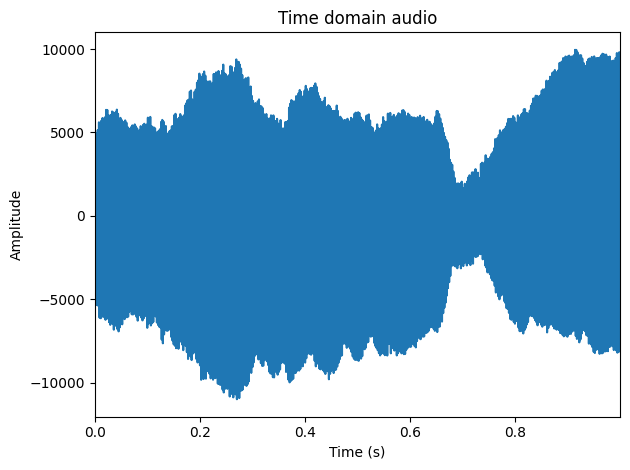
\includegraphics[width=\linewidth]{figs/time_domain_violin.png}
 \caption{One second time domain violin sample.}
\end{figure}

\begin{figure}[h]
 \centering
 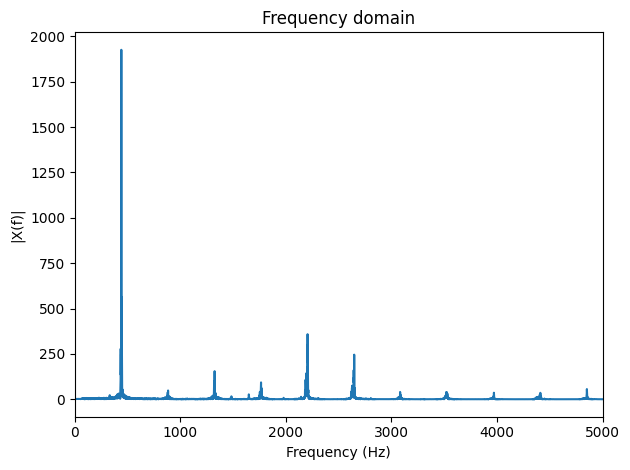
\includegraphics[width=\linewidth]{figs/frequency_doimain_violin.png}
 \caption{TThe same sample in frequency domain.}
\end{figure}

s the figures show, there is a main frequency that defines the pitch of the sound, along with many other frequencies that allow the ear to identify the instrument and distinguish between different kinds of sounds.

\subsubsection{Audio digitalization}

A microphone converts a pressure wave into an electrical waveform. However, in computational music, the audio signal must be discretized to be represented as a digital audio file. The primary process for digital audio representation is sampling.

Sampling consists of recording a sequence of wave amplitudes at fixed intervals. For example, if a sound is recorded using a sampling rate of 22,100 Hz, it means that the computer will capture 22,100 audio samples per second.

\begin{figure}[h]
 \centering
 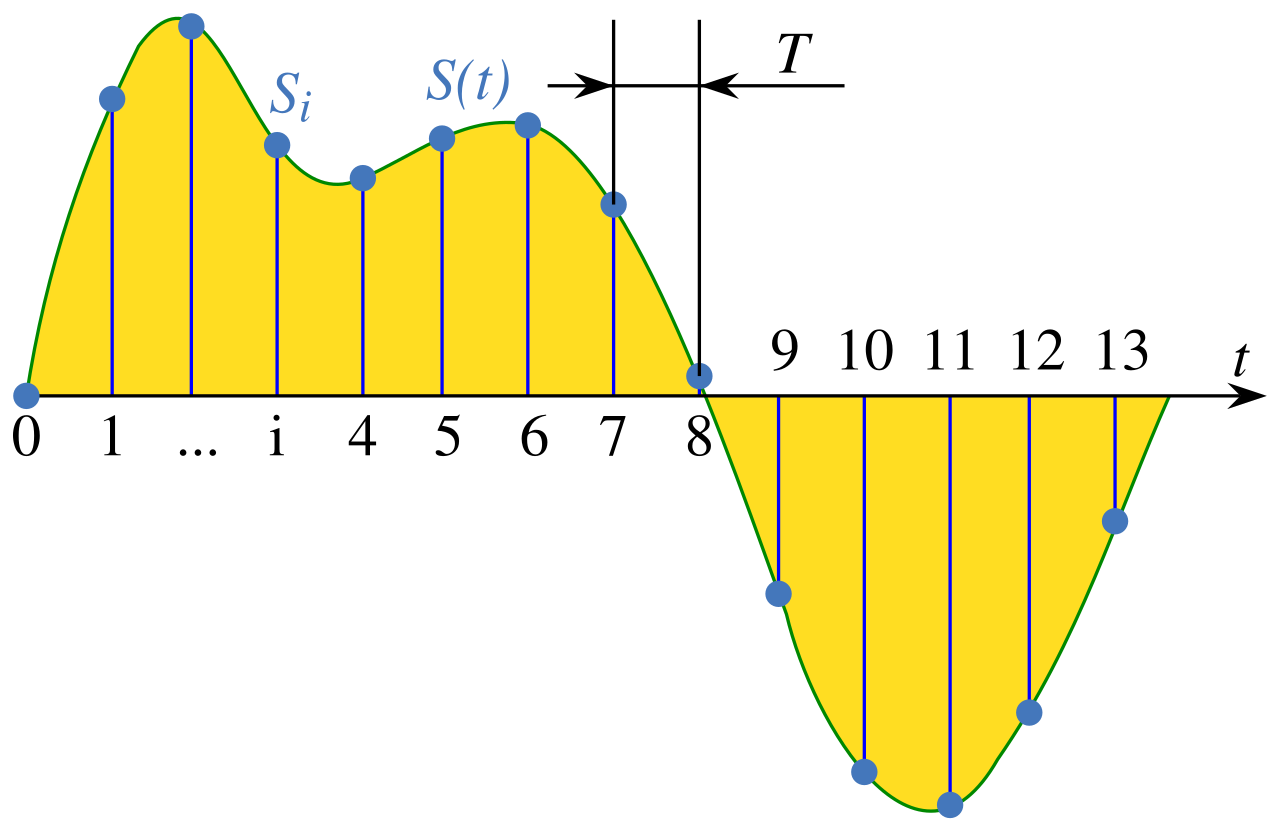
\includegraphics[width=\linewidth]{figs/signal_sampling.png}
 \caption{Signal sampling. Source: \cite{usp:logo}}
 \Description{Sinal sampling.}
\end{figure}

This approach is very efficient because human hearing can detect frequencies between 20 Hz and 20,000 Hz. However, for most musical sounds, the maximum frequency is typically below 10 kHz (in fact, even a violin — one of the highest-pitched instruments — reaches only around 3,500 Hz). And according to the Nyquist-Shannon Theorem, to properly sample a periodic signal, the sampling rate must be at least twice the frequency of the highest component of the signal.

Thus, 22,100 Hz can be a good sampling rate for recording music while saving disk space. However, if the goal is to cover the full range of human hearing, higher rates, such as 44,200 Hz, can also be used.

Note that with this process, all sound elements highlighted before, can be recorded and reprocedure later.

\subsubsection{Sound synthesis}

After the development of sound recording techniques, musical computation evolved toward the creation of artificial waveforms. Of course, before digital audio synthesis, there were several techniques that allowed analog synthesis. However, the underlying idea is essentially quite similar.

In summary, audio synthesis techniques can be divided into three basic types:

\begin{itemize}
\item Additive synthesis: Perhaps the most straightforward idea from a mathematical point of view. It consists of generating each frequency component of a desired timbre separately and then summing them. In fact, it is more like a weighted sum, since each component is weighted according to its contribution to the timbre. A normalization step is commonly applied after the process to avoid amplitude overload.

\item Subtractive synthesis: The opposite of the previous technique, but historically more common due to its effectiveness. In short, it consists of taking a complex waveform, rich in harmonics, and applying various filters to obtain the desired sound. It is more empirical than additive synthesis (which is based on spectral analysis), but simpler to implement and less computationally intensive. Typically, the original waveforms are complex ones such as the sawtooth wave, square wave, or triangular wave.

\item FM synthesis: Another empirical approach to sound synthesis, which will be addressed in detail in a later section. In short, it consists of altering a simple waveform by applying a high-frequency modulation, not to the generated waveform itself, but directly to the frequency parameter of the carrier oscillator. This kind of distortion of the base frequency produces mirrored harmonics that enrich the timbre of the sound. It is up to the musician to choose the appropriate parameters to produce the desired timbre.
\end{itemize}

There are many other techniques that could be mentioned; however, these three represent the most direct forms of synthesis, or the most purely mathematical ones, in the sense that they do not require manipulation of pre-recorded audio.

\subsubsection{ADSR Audio envelop}

Another important technique for achieving good results is the so-called “Attack, Decay, Sustain, and Release (ADSR) envelope”, which consists of applying a multiplicative function to the waveform, altering only its amplitude.

The basic idea is to control the sound intensity by simulating the natural behavior of acoustic sounds. Typically, an ADSR envelope is defined as a function with a domain between 0 and 1, which is applied to the generated waveform:

\begin{figure}[h]
 \centering
 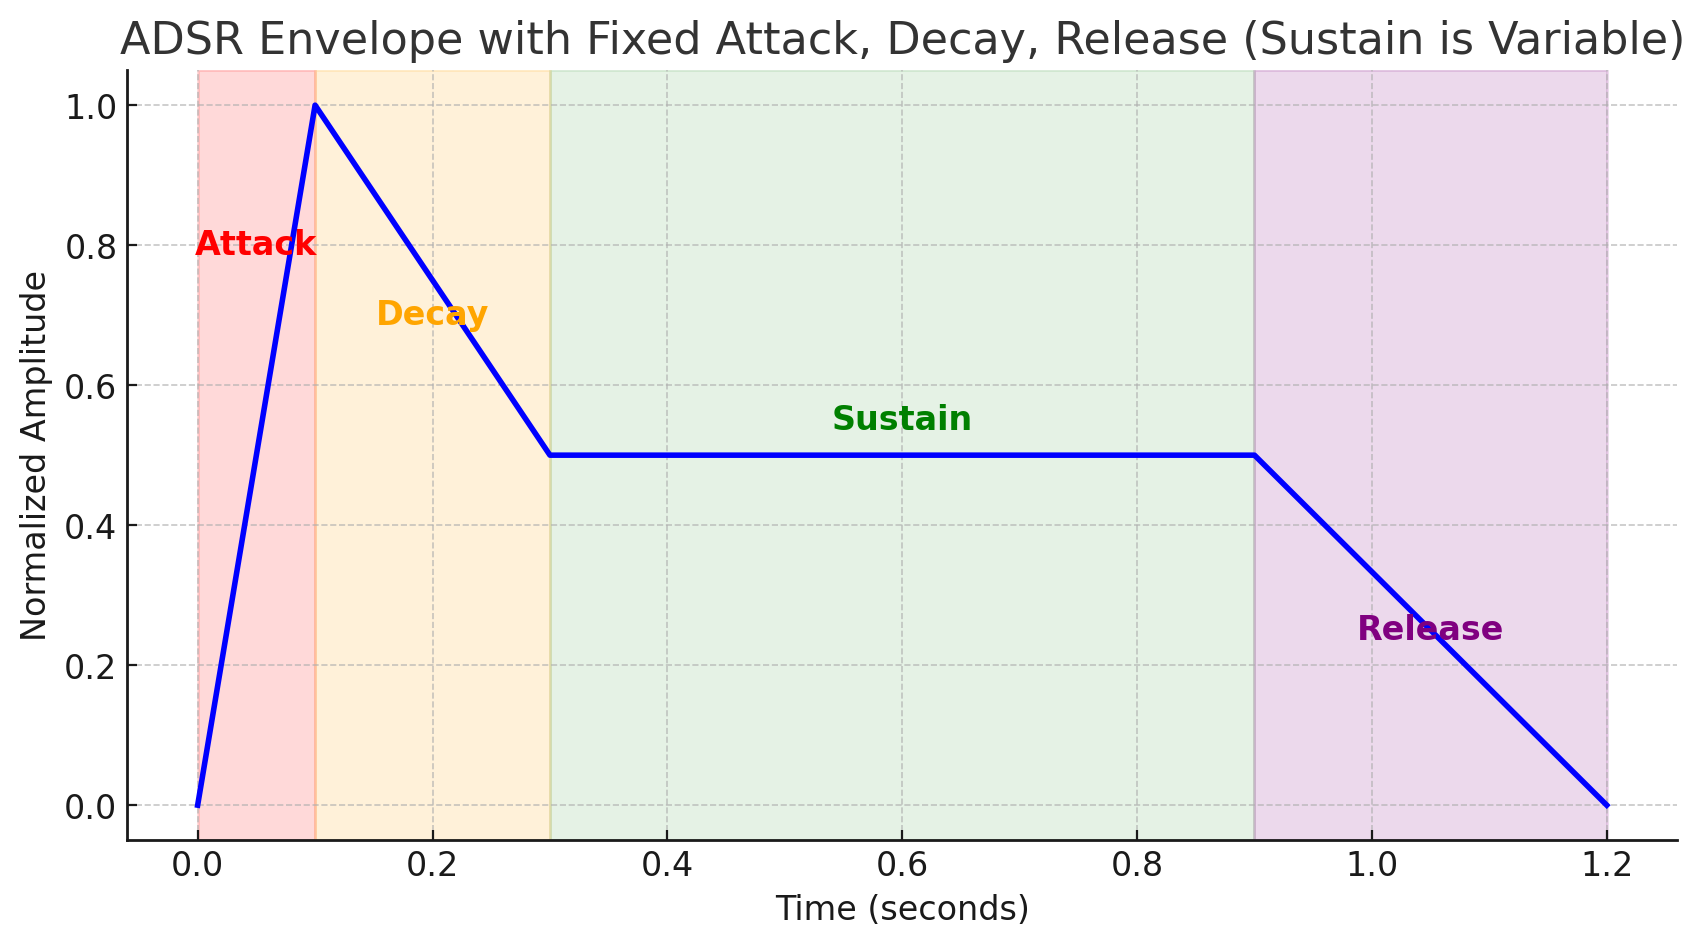
\includegraphics[width=\linewidth]{figs/adsr.png}
 \caption{ADSR linear envelop.}
 \Description{ADSR linear envelop.}
\end{figure}

The ADSR envelope can be understood as an amplitude function:

\[
y(t) = e(t) \cdot s(t)
\]

Where:

\begin{itemize}
\item \( s(t) \): the raw generated sound wave.
\item \( e(t) \): the ADSR envelope function (normalized amplitude ranging from 0 to 1).
\item \( y(t) \): the resulting sound.
\end{itemize}

Although real audio samples can show a wide variation of envelope behaviors, it is common practice to use a linear function to achieve the goal, since the human ear is more sensitive to abrupt changes and to relative differences. However, for longer variations, the ear can still perceive the change, which is why some synthesizers allow the use of exponential or logarithmic functions as well.

\subsection{FM Synthesis}

As shown in the previous sections, one of the most popular sound synthesis techniques is Frequency Modulation Synthesis (FM Synthesis), which was introduced by John M. Chowning in his famous paper “The Synthesis of Complex Audio Spectra by Means of Frequency Modulation”, published at the Stanford Artificial Intelligence Laboratory.

Chowning explored the effects of frequency modulation when applied with high frequencies, close to the audible range, instead of the traditional use of inaudible frequencies.

In fact, the concept of frequency modulation was already well known before this paper; however, it had been used mainly in radio transmission of music or to apply slight distortions through low-frequency oscillators (LFOs), producing effects such as vibrato.

As Chowning himself pointed out in his paper, when the technique is applied to vary the frequency of the carrier wave through a high-frequency modulator wave, it “results in a surprising control of audio spectra” (Chowning).

In summary, considering only two oscillators (the main one, called the carrier, and the modulator) the instantaneous frequency of the output audio can be expressed by the following function:

\[
f(t) = f_c + I \cdot \sin(2\pi f_m t)
\]

Where:

\begin{itemize}
\item \( f(t) \): the instantaneous frequency of the generated sound wave.
\item \( f_c \): the original frequency of the carrier wave.
\item \( I \): the modulation index, which defines the intensity of the modulation (the greater the value, the more harmonics are generated).
\item \( f_m \): the frequency of the modulator wave (which determines the spacing of the harmonics).
\item \( t \): the time variable.
\end{itemize}

The most important point, however, is that this simple manipulation results in symmetric sidebands around the carrier frequency, spaced at multiples of \( f_m \).

For a more intuitive understanding, if a carrier frequency \( f_m \) is modulated by a frequency \( f_m \), the resulting spectrum will contain:

\[
f_c \pm n f_m
\]

For example, by choosing \( f_c = 440 \) and \( f_m = 220 \), the resulting wave will contain frequency components such as 220 Hz, 440 Hz, 660 Hz, 880 Hz, and so on, with decreasing amplitudes (the amplitudes follow the Bessel coefficients, but this discussion is beyond the scope of this article).

The last important characteristic of Frequency Modulation Synthesis concerns the ratio between the carrier frequency and the modulator frequency \( f_c / f_m \), since this ratio directly influences the perceived audio result.

This ratio determines whether the generated harmonics align with the natural harmonic series (widely used by musicians) or not:

\begin{itemize}
    \item If the ratio is an integer number, the harmonic sidebands (in the spectral view) will appear as integer multiples of \( f_c \), generating harmonic sounds similar to those of real instruments (consistent with traditional music theory).
    \item If the ratio is not an integer value, the harmonic sidebands will not align perfectly with \( f_c \), and the generated sound may appear metallic or dissonant (this effect is useful for creating sounds such as bells or for producing special audio effects).
\end{itemize}

\subsection{Audio comparison}

The task of audio comparison is not straightforward, especially when the goal is to achieve equality in terms of human perception. It can be complex, computationally demanding, and inherently subjective.

However, as described in the section on timbre, one intuitive and efficient way to approach this problem is by comparing the audio in its spectral representation, since timbre is precisely defined by this combination of frequencies.

That said, this approach alone is not sufficient, because the Fourier Transform considers the entire audio signal at once, mixing different parts of a sound sample. For example, if a sample contains three different pitches in sequence, its frequency-domain representation will show them simultaneously, which may give the impression that the timbre is a mixture of all these pitches (similar to a chord rather than a sequence).

In fact, according to Claesson (2019), FFT-based spectral comparison is valid but only a part of the solution. He highlights the following additional metrics:

\begin{itemize}
    \item FFT Distance: This consists of computing the Fast Fourier Transform of the two samples being compared and then calculating the normalized Euclidean distance between them (the maximum distance is 1, and the minimum is 0).
    \item Short Time Fourier Transform (STFT) Distance: Equivalent to the FFT Distance, but calculated over short, overlapping slices of the sample, which provides time-localized spectral information.
    \item Log-Mel Spectogram Distance: Similar to the previous metrics, but based on the Log-Mel Spectrogram, which is essentially an adaptation of the FFT spectrum that incorporates human auditory perception. In summary, the Log-Mel Spectrogram is obtained by computing the STFT, mapping the frequencies onto the Mel scale (explained later in this document), and finally projecting the amplitudes onto a logarithmic scale.
\end{itemize}

In addition to these three metrics, Claesson also recommends the use of Euclidean Distance of the Envelope to compare audio envelopes. This approach can be very useful, but since this work is focused on the similarity between original and synthesized audio in terms of timbre, the envelope comparison, while important for real-world applications, falls outside the scope of the present study.

\subsubsection{Mel-Scale Representation}

The Mel scale was proposed by Stevens, Volkmann, and Newman in 1937 (Claesson, 2019), and its main purpose is to reflect the human perception of frequency.

The key difference from the linear scale is that, as the values on the scale increase, the perceptual difference between two adjacent points becomes smaller (and the corresponding difference in hertz is also reduced).

In fact, the Mel scale maps linear frequencies onto a logarithmic scale. A frequency \( f \) s converted to the Mel scale through the following formula:

\[
\text{Mel}(f) = 2595 \log_{10} \left( 1 + \frac{f}{700} \right)
\]

For a better understanding of this conversion, consider the following graph, which compares the linear hertz scale with the Mel scale:

\begin{figure}[h]
 \centering
 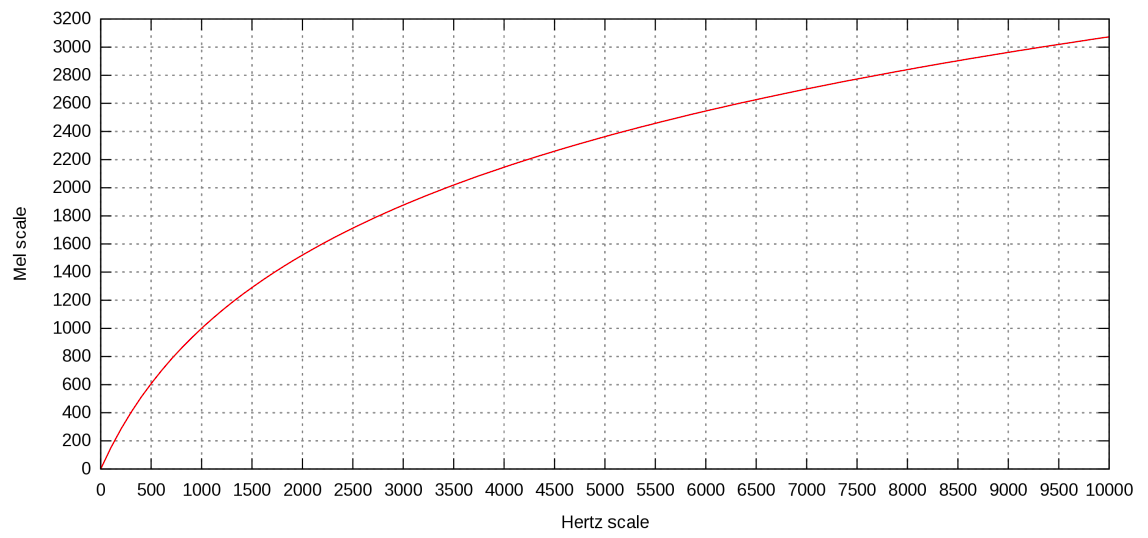
\includegraphics[width=\linewidth]{figs/mel_scale.png}
 \caption{Comparision between linear hertz scale and Mel scale (Claesson, 2019).}
 \Description{Comparision between linear hertz scale and Mel scale.}
\end{figure}

It is a very useful metric for audio comparison, as it takes into account the human auditory perception of frequency.

\subsection{Convolutional Neural Networks (CNN)}

\subsubsection{2D Convolutional Neural Networks}

In summary, a convolutional neural network is based on the idea of filters.

Before the introduction of CNNs, was already known that many computer vision problems can be solved through the evaluation of image features, which become more evident depending on the filters applied.

For exampe, to classify differe animals, just the silhouettes can be enough. Of course, the fewer features considered, the higher the chance of mistakes, but, as popular saying goes: “if it walks like a duck, quacks like a duck, flies like a duck… it’s a duck!”. That’s the basic idea.

So, the CNNs was concept in such a way that several layers of filters of fixed size (chosen by the network designer) are defined, in addition to some pooling layers (which will be discussed later).

These filter layers are also organized according to the designer’s choices (usually based on many experiments) and can be applied in sequence, in parallel, using different combinations, and so on.

However, it is important to note that the filters serve as the link between the different representations of the input image built within the network.

That is, although the network still takes an image as input, and although this image is processed to extract the various features needed for the problem, there are no dense interconnections between these image representations.

In fact, what interposes between one image representation and another is precisely a CNN filter. And even this filter is not densely connected to the image representations.

In practice, the filter is not connected to any specific part of the image. Instead, it is “slid” across the image, performing a Hadamard multiplication (element-wise product) between the filter and each frame of the image (of the same size), producing, as output, a “new filtered image” (multiplication, element by element, of two matrices of the same size, with a final sum of all elements — and, typically, with the application of an activation function to the result).

Visually, the work can be represented as follows:

\begin{figure}[h]
 \centering
 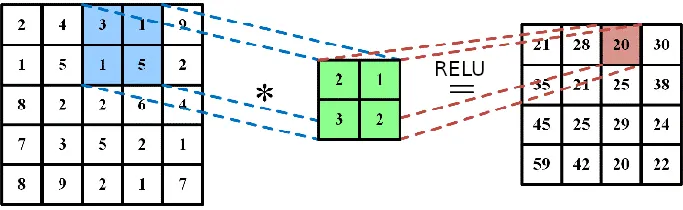
\includegraphics[width=\linewidth]{figs/hadamard_product.png}
 \caption{Hadamard product between a filter and an input layer slice (Adapted from ResearchGate, 2024)).}
 \Description{Hadamard product between a filter and an input layer slice.}
\end{figure}

And it is precisely from this sliding operation that the network architecture takes its name, since this action corresponds to the mathematical operation of convolution:

To an inout image \( I \), a filter (or Kernel) \( K \), the convolution output \( O \), in a point \( (i,j) \) is given by:

\[
O(i,j) = \sum_{m=0}^{M-1} \sum_{n=0}^{N-1} K(m,n) \times I(i+m, j+n)
\]

Where:

\begin{itemize}
\item \( K(m,n) \): the filter element on position \( (m,n) \).
\item \( I(i+m, j+n) \): the element of the input on position of current window.
\item \( M, N \): the height and width of the filter.
\item \( O(i,j) \): the output element on position \( (i,j) \).
\end{itemize}

Thus, CNNs can perform image filtering while at the same time reducing the amount of memory required compared to traditional fully connected feed-forward networks (because memory is allocated only for the filters and their results, rather than for each individual interconnection weight).

After extracting the necessary features from the data, a small traditional dense (multi-layer) network is added after the convolution (and pooling) layers. This dense network is responsible for identifying the patterns required to predict the target variable (whether for classification or regression).

A CNN is typically divided into two stages. The first stage consists of the application of filters (along with pooling layers), while the second stage applies a fully connected network. In this second stage, the output of the first part undergoes a flattening process so that it can be used as input to the fully connected layers, which handle the usual tasks of classification or regression.

\section{Related work}

\section{Proposed approach}

The overall idea of the project can be summarized as follows:

\textit{Use AI to guide an FM synthesizer in simulating any instrument.}

Or, in a more detailed explanation:

\textit{Use a Convolutional Neural Network (CNN) to analyze an instrument's sound sample and predict the correct parameters for an FM synthesizer to re-synthesize the ``same'' sound, enabling the synthesizer to simulate that instrument playing any song.}

However, this idea is still quite abstract and broad. Therefore, consider the following steps to achieve the project's goal:

\begin{enumerate}
\item Implement a simple FM synthesizer, which can later be used both to generate the dataset and to test the ability to re-synthesize a sound.
\item Generate an audio dataset with random audio samples, each created by randomly selecting FM synthesizer parameters, essentially recording tuples of (parameter values; audio sample).
\item Train a CNN to predict the correct parameters for the same FM synthesizer, given only an audio sample.
\item Evaluate the model's results using the NSynth dataset to test its generalization capabilities.
\end{enumerate}

Frequency Modulation Synthesis was chosen because it is one of the most common and effective methods for generating audio samples, owing to its simplicity and low computational cost.

This technique became extremely popular in the 1980s, when Yamaha released the Yamaha DX7 synthesizer, and in the 1990s it became a standard for many commercial synthesizers, and it is still used today in the production of electronic music (Claesson, 2019).

However, the effective use of this technique depends on advanced knowledge to select the right parameters for generating good results, which can involve thousands of parameters.

Therefore, the ability to simplify parameter selection constitutes a strong justification for this study, and AI models appear as an affordable way to learn the right patterns for controlling an FM synthesizer.

The basic idea is that a model can be produced to guide an FM synthesizer in mimicking any sound, thereby optimizing the effort to compose electronic music.

Furthermore, in terms of computational cost, using an AI model to predict parameters and guiding an FM synthesizer is much more effective than applying a Generative Neural Network to generate the audio. Additionally, a synthesizer can be best applied in real-time composition and electronic musician performance.

\subsection{Training the CNN}

As described in the ``Theoretical Background`` section, the main characteristic of the sound that should be reproduced to achieve the main work goal is the ``timbre``, which is defined as the combination of frequencies present in the sound.

It is clear that techniques such as filtering, Fourier Transform, and etc, could be used to extract the timbre components from an audio signal, but it is not enough to control an FM Synthesizer. In fact, the FM Synthesis controlling is, normally, an experimental process involving trial and error.

Additionally, as described before, each FM Synthesis operator produces additional frequency components in the signal, and there is no practical method to predict the correct parameter settings, but, as a mathematical function, it is easy to see that this synthesis pattern can be easily approximated using AI models.

Thus, the current work aims to use a CNN model, since it is a very effective method for learning patterns, respecting the internal data structure, and without requiring a lot of preprocessing work.
In other words, a CNN can simultaneously learn the time-dependent aspects of an audio signal and can act as a pattern extractor, by applying a sequence of filtering operations, allowing the use of the raw audio format as input.

And so, to train the CNN model, a generated random dataset will be used, which main advantage is that it contains both the audio signal and the expected parameters for generating each sample sound. Therefore, the training process is straightforward and should yield good performance.

The figure below presents the overall scheme for this training process.

\begin{figure}[h]
 \centering
 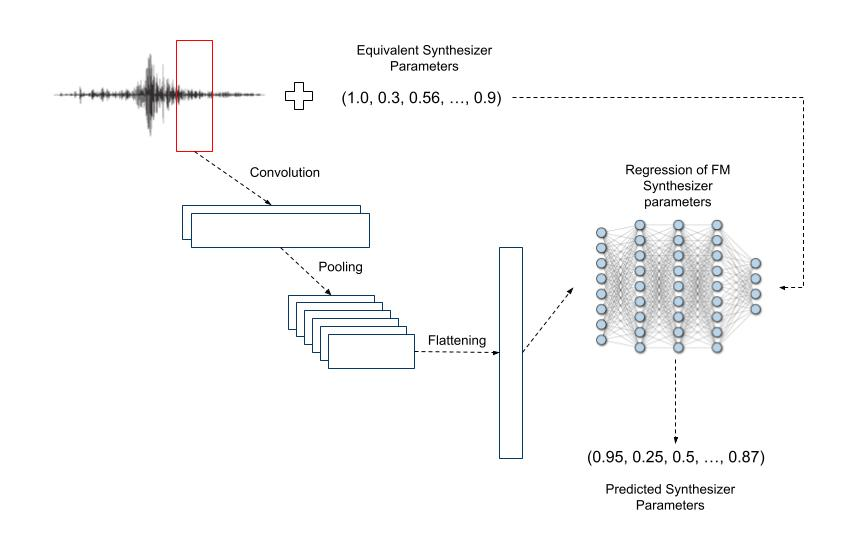
\includegraphics[width=\linewidth]{figs/cnn_simple_training.jpg}
 \caption{The CNN training scheme.}
 \Description{The CNN training scheme.}
\end{figure}

\subsubsection{Evaluating Results}

As introduced in the ``Theoretical Background'' section, the following audio similarity metrics will be used in this work:

\begin{itemize}
\item FFT distance: Used to compare the frequency components present in an audio signal.
\item STFT distance: Used to compare the variation of frequency components over time.
\item Log-mel-spectrogram distance: Used for a similar purpose as FFT distance, but typically models human cognitive pitch perception more accurately.
\end{itemize}

These metrics will be applied to perform a final test of the model's generalization capability.

The proposed approach is, after the model training, to use another external dataset, the Google NSynth dataset, which is better described below, and will be used in order to determine whether the model is able to re-synthesize real instruments, following the steps outlined below:

\begin{enumerate}
\item Train the model with the random generated dataset
\item Test the model with the NSynth dataset
\item Re-synthesize the NSynth dataset using the predicted parameters
\item Calculate the audio similarity metrics
\item Evaluate the results
\end{enumerate}








\section{Experiments}

\subsection{Setup}

\subsubsection{Implemented FM Synthesizer}

There are several well-known FM synthesizers on the market, but most are not open-source. Additionally, commercial synthesizers often have a vast number of parameters that can be used to control the audio production process. For example, Native Instruments' FM8 can use around 1,000 parameters (Claesson, 2019), and Teenage Engineering’s OP-1 synthesizer can be configured with up to $10^{76}$ parameters (Claesson, 2019).

This incredibly large number of parameters is intended to give users fine-grained control over the generated audio, allowing for a wide variety of pitches (simulating a broad range of instruments and even non-instrument sounds, such as bird songs or car horns, among others).

However, since the scope of this project is not focused on a commercial solution but rather on research purposes, a simple FM synthesizer will suffice.

Therefore, this work will implement a basic FM synthesizer with only 6 operators, inspired by the classic Yamaha DX7, which was one of the most disruptive milestones in the history of electronic music composition. In fact, this simple setup is enough to cover all FM synthesis theories and achieve good performance during AI model evaluation.

In summary, the implemented synthesizer will consist of:

\begin{itemize}
\item 5 modulator operators
\item 1 carrier operator
\item 1 ADSR envelope
\item 2 synthesis algorithms (one completely serial, and another with 3 serial operators followed by 2 parallel operators)
\end{itemize}

The synthesizer will be implemented in Python, using the NumPy library for numerical processing and the SciPy library for audio file generation (in addition to the python-soundfile library).

The figure below presents the FM Synthesizer algorithms:

TODO

To summarize, the implemented synthesizer renders the audio signal according to the following steps:

\begin{enumerate}
\item Generate each operator signal, applying it to vary the phase of the next operator in the sequence (a completely FM synthesis also varies the frequency, but, as the Yamaha DX7, it only varies the phase, for simplicity, and to avoid complex noise treatment). All signals are rendered using a 48 kHz sample rate.
\item Combine the output of each operator according to the synthesis algorithm (when there are parallel operators, they are summed).
\item Apply the ADSR envelope to the signal.
\item Downsample the signal to 16 kHz (applying a low-pass filter to avoid aliasing).
\end{enumerate}

And it is important to highlight that the high sample rate of 48 kHz was chosen to allow the FM synthesis to work well enough, since at high frequencies there is a risk of obtaining aliasing and noise (due to the extremely high frequency components generated by the normal spacing of the FM operators). Furthermore, the low-pass filtering, used to downsample, is also useful to prevent the aliasing problem.

\subsubsection{Generating the dataset}

This project will use two datasets, each for a specific purpose: the first is the generated dataset, used for training, and the second is the NSynth dataset, used to evaluate the model's generalization capabilities.

One of the most challenging steps in the KDD process is obtaining and processing data. However, for the purposes of this work, an effective approach can be used. Similar to Claesson's approach (Claesson, 2019), since the goal is to achieve good control over the synthesizer parameters, it is sufficient to generate many samples of synthesizer parameters and their respective audio outputs.

Therefore, the main dataset will consist of 5,000 samples generated by the implemented FM synthesizer, with the following characteristics:

\begin{itemize}
\item 5,000 samples
\item 4 seconds in duration
\item Monophonic samples (1-channel audio)
\item 16 kHz audio sample rate (the synthesizer will generate samples at 48 kHz, but they will be downsampled to 16 kHz to be compatible with the NSynth dataset)
\item Pitches varying between 20 Hz and 6,000 Hz
\item Random ADSR envelopes
\end{itemize}

The expectation is to achieve a level of learning where the model can accurately predict the parameters for a wide range of sounds that can be generated by the implemented FM synthesizer.

\subsubsection{External dataset}

In addition to the generated dataset, an external dataset called NSynth, from Google's Magenta project, will be used.

This dataset has a similar configuration to the generated one, and its main purpose is to evaluate the generalization capabilities of the model. This is because it contains many real instrument samples, including both acoustic and electronic instruments (as well as some synthetic sounds generated by professional synthesizers), which the model has never seen before.

Only the test set of the NSynth dataset will be used, with the following characteristics:

\begin{itemize}
\item 4,096 samples
\item 4 seconds in duration
\item Monophonic samples (1-channel audio)
\item 16 kHz audio sample rate
\item 11 instrument families
\item Pitches ranging from 27.5 Hz to 4,186.01 Hz
\item The envelope includes a sustain of up to 3 seconds and a decay of 1 second
\end{itemize}

\subsubsection{CNN Architecture}



\subsection{Plan}
-dataset
-protococlos de avaliação

\subsection{Results}


\section{Conclusion}





\section{Tables}

The ``\verb|acmart|'' document class includes the ``\verb|booktabs|''
package. Table captions are placed {\itshape above} the table.

% Please note that table captions should be placed ABOVE the table
\begin{table}
  \caption{Frequency of Special Characters}
  \label{tab:freq}
  \begin{tabular}{ccl}
    \toprule
    Non-English or Math&Frequency&Comments\\
    \midrule
    \O & 1 in 1,000& For Swedish names\\
    $\pi$ & 1 in 5& Common in math\\
    \$ & 4 in 5 & Used in business\\
    $\Psi^2_1$ & 1 in 40,000& Unexplained usage\\
  \bottomrule
\end{tabular}
\end{table}


\section{Math Equations}
You may want to display math equations in three distinct styles:
inline, numbered or non-numbered display.  Each of the three are
discussed in the next sections.

Inline equations: 
\begin{math}
  \lim_{n\rightarrow \infty}x=0
\end{math},
set here in in-line math style.

Numbered equation, shown as an inline equation above:
\begin{equation}
  \lim_{n\rightarrow \infty}x=0
\end{equation}

Now, we'll enter an unnumbered equation:
\begin{displaymath}
  \sum_{i=0}^{\infty} x + 1
\end{displaymath}
and follow it with another numbered equation:
\begin{equation}
  \sum_{i=0}^{\infty}x_i=\int_{0}^{\pi+2} f
\end{equation}

\section{Figures}

The ``\verb|figure|'' environment should be used for figures. One or
more images can be placed within a figure. If your figure contains
third-party material, you must clearly identify it as such, as shown
in the example below.

% Please note that figure captions should be placed BELOW the figure

\begin{figure}[h]
  \centering
  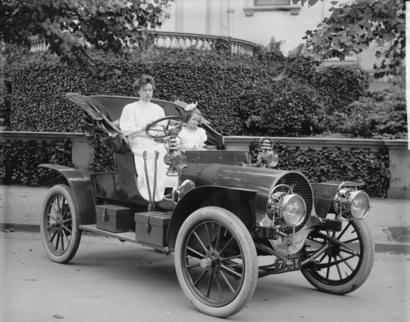
\includegraphics[width=\linewidth]{figs/sample-franklin}
  \caption{1907 Franklin Model D roadster. Photograph by Harris \&
    Ewing, Inc. [Public domain], via Wikimedia
    Commons. (\url{https://goo.gl/VLCRBB}).}
  \Description{A woman and a girl in white dresses sit in an open car.}
\end{figure}

Your figures should contain a caption which describes the figure to
the reader.

Figure captions are placed {\itshape below} the figure.

Every figure should also have a figure description unless it is purely
decorative. These descriptions convey what’s in the image to someone
who cannot see it. They are also used by search engine crawlers for
indexing images, and when images cannot be loaded.

A figure description must be unformatted plain text less than 2000
characters long (including spaces).  {\bfseries Figure descriptions
  should not repeat the figure caption – their purpose is to capture
  important information that is not already provided in the caption or
  the main text of the paper.} For figures that convey important and
complex new information, a short text description may not be
adequate. More complex alternative descriptions can be placed in an
appendix and referenced in a short figure description. For example,
provide a data table capturing the information in a bar chart, or a
structured list representing a graph.  For additional information
regarding how best to write figure descriptions and why doing this is
so important, please see
\url{https://www.acm.org/publications/taps/describing-figures/}.


\begin{acks}
This work is supported by \textit{Coordenação de Aperfeiçoamento de Pessoal de Nível Superior}~(CAPES), \textit{Conselho Nacional de Desenvolvimento Científico e Tecnológico}~(CNPq), grants 406417/2022-9, 102475/2024-5, and 312209/2022-3, and \textit{Fundação de Amparo à Pesquisa do Estado de São Paulo}~(FAPESP), grant 2020/09835-1~(CPA IARA). 
\end{acks}


%%
%% Print the bibliography
%%
\printbibliography



\end{document}
\endinput
%%
%% End of file `sample-sigconf-biblatex.tex'.

Claesson